\documentclass{article}

\usepackage{geometry}
\usepackage{amsmath}
\usepackage{graphicx}
\usepackage{listings}
\usepackage{hyperref}
\usepackage{multicol}
\usepackage{fancyhdr}
\pagestyle{fancy}
\hypersetup{ colorlinks=true, linkcolor=black, filecolor=magenta, urlcolor=cyan}
\geometry{ a4paper, total={170mm,257mm}, top=20mm, right=20mm, bottom=20mm, left=20mm}
\setlength{\parindent}{0pt}
\setlength{\parskip}{1em}
\renewcommand{\headrulewidth}{0pt}
\lhead{Competitive Programming - Arkavidia V}
\fancyfoot[CE,CO]{\thepage}

\begin{document}

\begin{center}
    \section*{D. DVD} % ganti judul soal

    \begin{tabular}{ | c c | }
        \hline
        Batas Waktu  & 1s \\    % jangan lupa ganti time limit
        Batas Memori & 64MB \\  % jangan lupa ganti memory limit
        \hline
    \end{tabular}
\end{center}

\subsection*{Deskripsi}

\begin{center}
    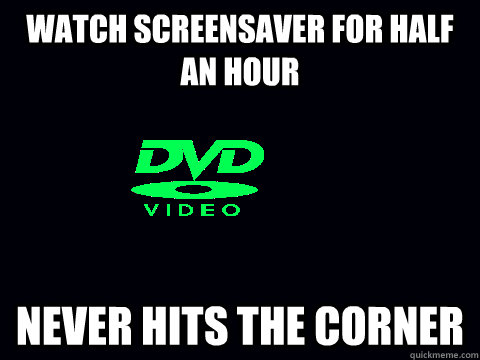
\includegraphics[width=200px]{meme}
\end{center}

Arvy sedang memandang layarnya yang berukuran $W \times H$ satuan.
Di layarnya, sedang berjalan \textit{screen saver} DVD.
Pada \textit{screen saver} ini, logo DVD bergerak lurus.
Ketika menyentuh sisi layar, logo DVD akan berubah warna dan memantul dengan sudut kedatangan sama dengan sudut pantulan (Secara formal, sudut yang dibentuk antara garis gerakan logo sebelum memantul dan sisi layar sama dengan sudut yang dibentuk antara garis gerakan logo sesudah memantul dan sisi layar).
Setiap kali memantul, logo DVD berubah warna.

Arvy lelah menonton \textit{screen saver} DVD yang terus memantul-mantul.
Ia menunggu-nunggu kapan logo DVD berhenti di pojok layar.
Ia mulai ragu apakah logo DVD akan berhenti di pojok layar.
Akhirnya ia memfoto gerakan logo DVD dua kali, di mana logo DVD di kedua foto masih memiliki warna yang sama. Kedua logo ini berada di koordinat $(x_1, y_1)$ dan $(x_2, y_2)$.

\subsection*{Format Masukan}

Baris pertama terdiri dari sebuah bilangan $T$ ($1 \leq T \leq 1.000$), menyatakan jumlah kasus uji.

$T$ baris berikutnya terdiri dari 4 bilangan bulat, yakni $W$, $H$, $x_1$, $y_1$, $x_2$, $y_2$ ($1 \leq W, H \leq 1.000.000.000$, $1 \leq x_1, x_2 \leq W$, $1 \leq y_1, y_2 \leq H$).

\subsection*{Format Keluaran}

Untuk tiap kasus uji, tuliskan \lstinline{YAY} jika logo DVD akan menyentuh koordinat tepat sudut layar TV, atau \lstinline{NAY} jika tidak.
\\

\begin{multicols}{2}
\subsection*{Contoh Masukan 1}
\begin{lstlisting}
TBD
\end{lstlisting}
\columnbreak
\subsection*{Contoh Keluaran 1}
\begin{lstlisting}
TBD
\end{lstlisting}
\vfill
\null
\end{multicols}

\subsection*{Penjelasan}
TBD.

\pagebreak

\end{document}